\newpage
\section{Classes and program functionality overview}
The GUI application is written in QT (c++). It contains of a main window which holds different kinds of widgets that can be dragged around. It also features a settings dialogue and a serial console for manually sending messages.
A class diagram can be seen in figure~\ref{fig:classdiagram}.
\par\bigskip
\begin{figure}[h]
	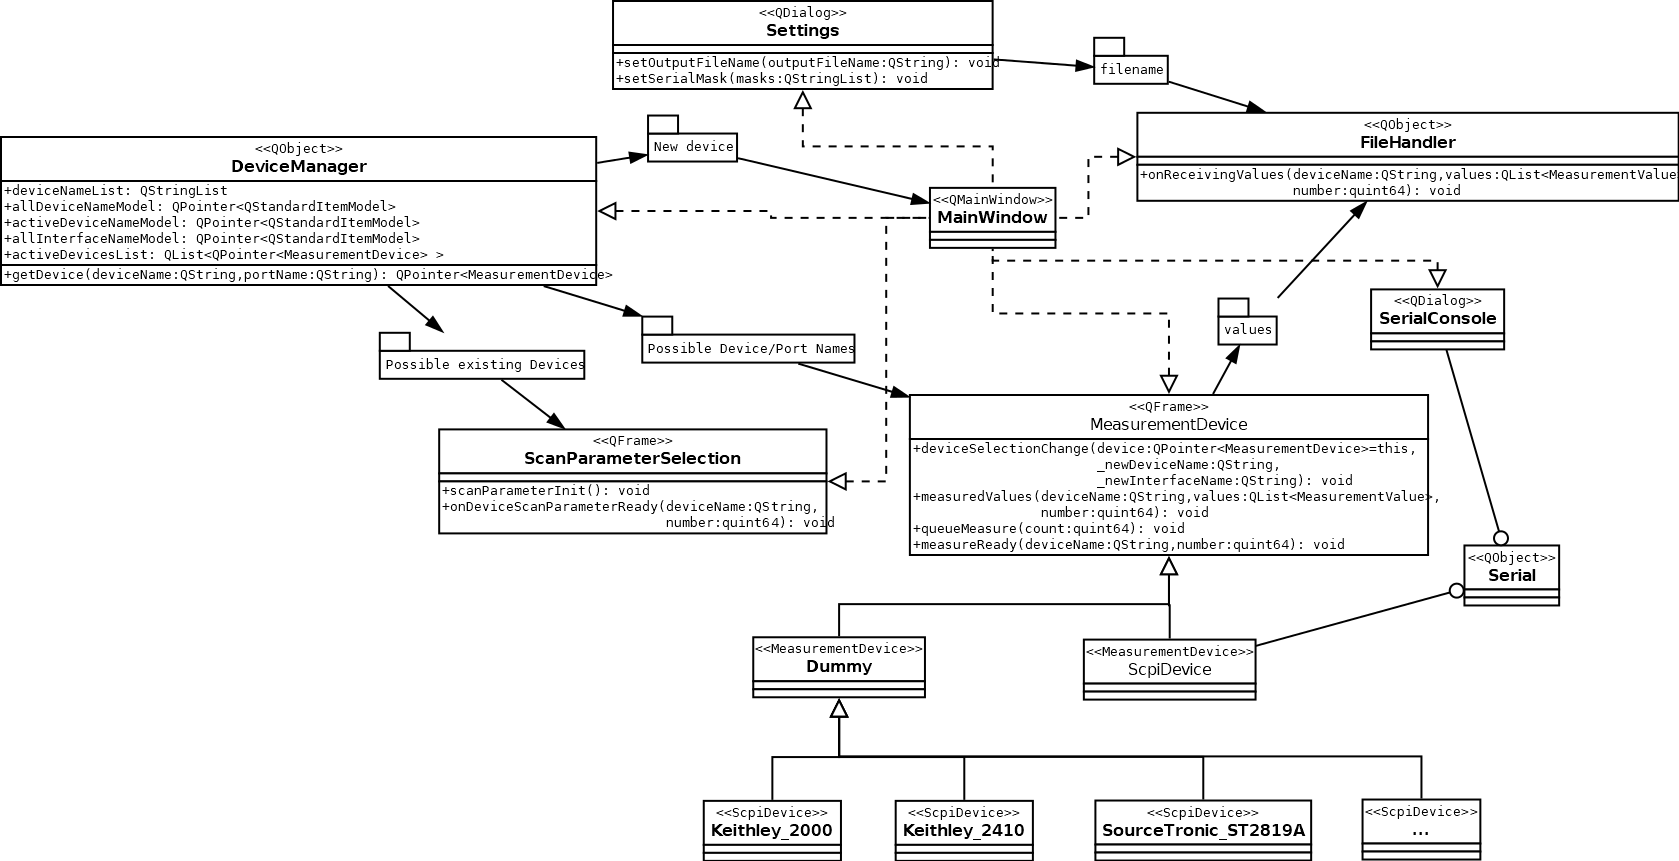
\includegraphics[width=\textwidth]{generalpurposecontrol.png}
	\caption{class diagram}
	\label{fig:classdiagram}
\end{figure}
\par\bigskip

The MainWindow class can contain objects of type MeasurementDevice and ScanParameterSelection in different areas of the GUI as can be seen in figure~\ref{fig:guicolored}.\par\bigskip

The MeasurementDevice is for itself a widget that has a graphical representation of the parameters one hardware device might have: a device name, port (address) and a table of values that can be written or read by the device, for example voltage or current. MeasurementDevice has abstract functions for starting measurements and sending the results to some other class and is therefore the parent class of all device classes. Polymorphism is used to store all different child classes inside the same layout in the main window.\par\bigskip

The ScanParameterSelection class is used to set write-enabled parameters to certain values or ramping them during a measurement. A previously instantiated device can be selected from the drop down menu in ScanParameterSelection thanks to the DeviceManager class which holds an overview of all instantiated device objects and providing the item models for the drop down menus etc. The ScanParameterSelection object tells the MeasurementDevice to write certain parameters during a measurement.\par\bigskip
\newpage

\begin{figure}[h]
	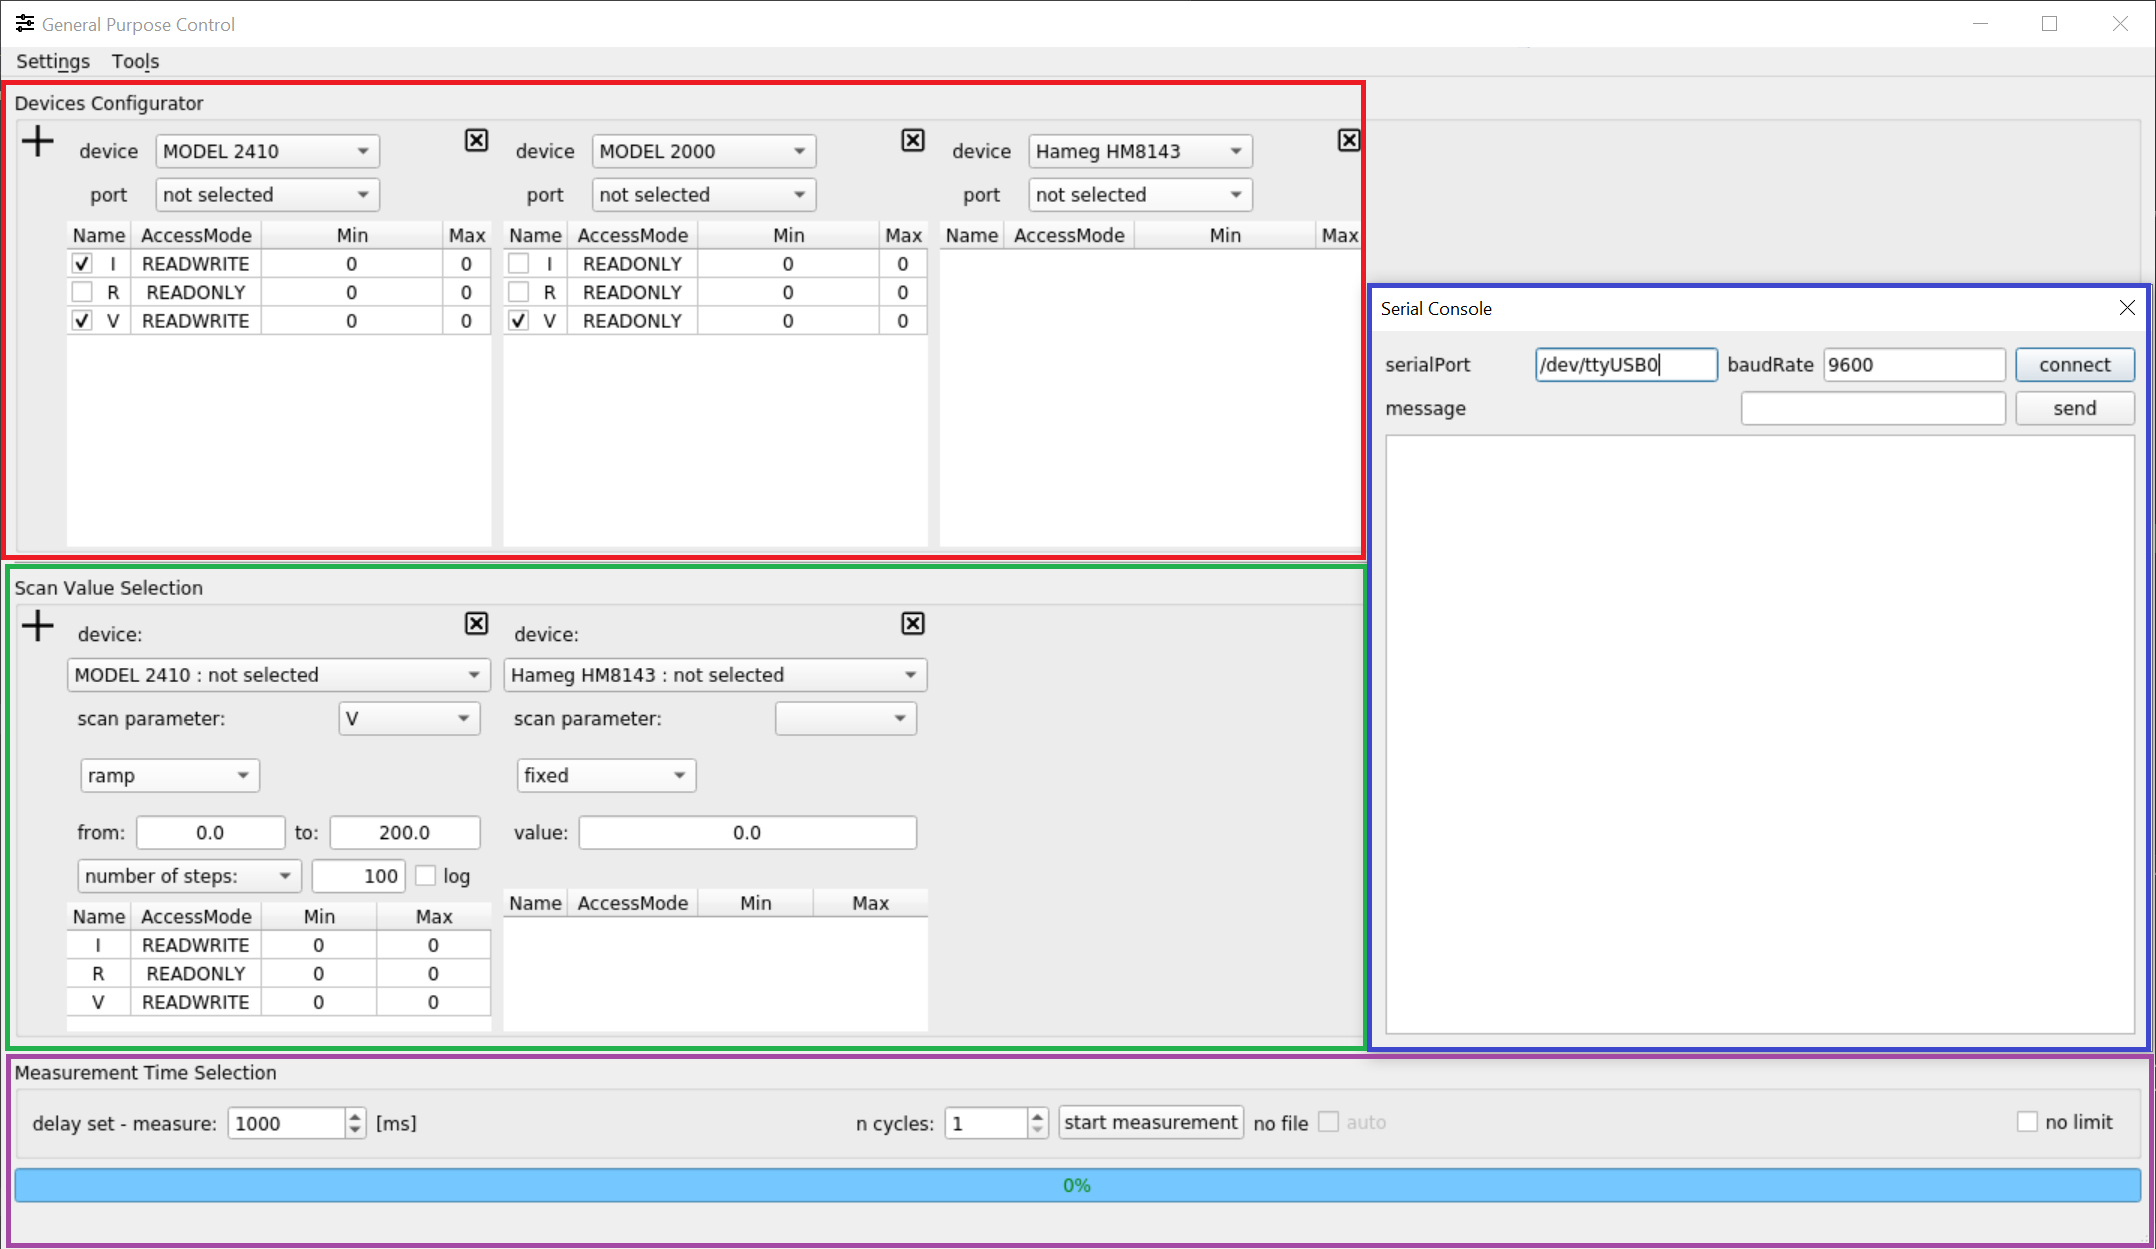
\includegraphics[width=\textwidth]{gui_all_colored.png}
	\caption{\\
		\color{Red}red\color{black}: Device selection area;\\
		\color{Green}green\color{black}: Scan parameter selection area;\\
		\color{Blue}blue\color{black}: Serial console pop-up dialog; \\
		\color{Purple}purple\color{black}: measurement / time selection and info area}
	\label{fig:guicolored}
\end{figure}
\par\bigskip

When a measurement is started in the main window by clicking 'start measurement' all ScanParameterSelection widgets create basically a nested loop. At each measurement step only one ramping parameter will be changed, allowing ramping of multiple parameters on multiple devices controlled by only one application. The progress of the whole measurement procedure is tracked by a progress bar which is calculated at each increment, showing the overall progress.
\par\bigskip

The main goal was to connect to tabletop lab devices via uart at first but other devices that use different serial connections can be used as well. However, the serial console that can be opened in the main window focuses on manually sending plain text messages via uart and displaying the received messages. This feature might be updated in the future to have more diverse features such as other serial interfaces and support for different device protocols (for example binary messages).\par\bigskip

Another feature is the settings dialogue which features a filter for port names to only allow for example "tty*" ports. It also features a file output selection where the user can select the file to which the measurements are written. This file will also be shown in the bottom area of the main window.
\par\bigskip

In the future the exact options inside ScanParameterSelection will probably change to provide more features. Also the settings will get updates depending on future features.